\documentclass[11pt,final]{article}
%\documentclass[11pt,draft]{article}

%%% Load some useful packages:
%% "New" LaTeX2e graphics support.
\usepackage{graphicx}
%%	using final option to force graphics to be included even in draft mode
%\usepackage[final]{graphicx}
%% Tell graphicx the default directory for all figures
%\graphicspath{{figures/final/}}

%% Enable subfigure support
\usepackage{subfigure}

%% Make subsubsections numbered and included in ToC
\setcounter{secnumdepth}{3}
\setcounter{tocdepth}{3}

%% Package to linebreak URLs in a sane manner.
\usepackage{url}

%% Define a new 'smallurl' style for the package that will use a smaller font.
\makeatletter
\def\url@smallurlstyle{%
  \@ifundefined{selectfont}{\def\UrlFont{\sf}}{\def\UrlFont{\small\ttfamily}}}
\makeatother
%% Now actually use the newly defined style.
\urlstyle{smallurl}

%% Define 'tinyurl' style for even smaller URLs (such as in tables)
\makeatletter
\def\url@tinyurlstyle{%
  \@ifundefined{selectfont}{\def\UrlFont{\sf}}{\def\UrlFont{\scriptsize\ttfamily}}}
\makeatother

%% Provides additional functionality for tabular environments
\usepackage{array}

%% Provides additional functionality for enumeration environments
\usepackage{enumitem}

%% Puts space after macros, unless followed by punctuation
\usepackage{xspace}

%% Make margins less ridiculous
\usepackage{fullpage}

%% Allows insertion of fixme notes for future work
\usepackage[footnote, nomargin]{fixme}

%%%% Turned off for tech report, should be turned on for research portfolio
%% Turn on double spacing
%\usepackage{setspace}
%\doublespacing

%% Make URLs clickable
%\usepackage[colorlinks, bookmarks=false]{hyperref}
\usepackage[colorlinks, bookmarks=true]{hyperref}

%% Since I'm using the LaTeX Makefile that uses dvips, I need this
%% package to make URLs break nicely
\usepackage{breakurl}

%%% End of preamble
\begin{document}

\title{Makahiki: A Serious Game Engine for Sustainability}
\author{A Research Proposal White Paper \\
\\
Yongwen Xu\\
Department of Information and Computer Science\\
University of Hawai`i \\
yxu@hawaii.edu\\
Version 0.1 \\
}
\date{June 2012}

%%% Create the title page from all the information above. Note that the
%%% titlepage is outside the front matter.
\maketitle

\section{Summary}

My research seeks to investigate how to build a customizable serious game engine for sustainability called Makahiki. It provides an open source, component-based, extensible framework for creating serious games for the purpose of education and behavioral change regarding energy, water, food, and waste generation and use. Different organizations configures the Makahiki framework to produce a ``challange instance'' with a specific set of game mechanics, user interface features, and experimental goals. Makahiki provides sophisticated instrumentation to support evaluation of how well the game mechanics supported the organization's goals for the challenge.

This white paper describes the Makahiki's research goal, system design, and experimental design on how to evaluate the effectiveness of the Makahiki as framework in developing serious games.

%% Contains introduction to the related work when used outside the
%% context of the dissertation proposal
\section{Introduction}

Sustainability education and conservation has become an international imperative due to the rising cost of energy, increasing scarcity of natural resources and irresponsible environmental practices. 
Over the past decade, running energy and water challenges have become a focal point for sustainability efforts at university, government, and industry campuses. Designers of those competitions have had three choices for information technology: (a) build their own custom in-house solution; (b) out-source to a commercial provider; or (c) use a "minimal tech" solution such as a web page and manual posting of data and results.

We developed a framework called Makahiki as a new choice: an extensible game engine for the development and evaluation of sustainability challenges. Makahiki has a unique feature set intended to foster more rapid innovation and development. These features include: (1) an open source license and development model which makes the technology available without charge and facilitates collaborative development and improvement; (2) support for an "ecosystem" of extensible, interrelated, customizable games and activities; (3) real-time game analytics and A/B testing for research and evaluation; (4) pedagogically organized and extensible learning activities; (5) a responsive user interface supporting mobile, tablet, and laptop displays; and (6) support for deployment to the cloud as an inexpensive option for hosting the competition.

The Makahiki framework will be used in 2012 by three organizations, namely, University of Hawaii at Manoa, Hawaii Pacific University, East West Center of University of Hawaii, to implement individually tailored sustainability challenges. 

\section{Research Goals}

There are two research goals in Makahiki: (a) provides an extensible framework to easily create engaging games for sustainability education and behavior change, and (b) provides an experimental test bed for Gamification research into the effectiveness of different game mechanics in the context of sustainability.

The challenges of creating a customizable game engine are:  (a) creating a new instance of Makahiki by selecting the games they want the system to support, and (b) extending Makahiki by writing new game components, and (c) supporting ease of use by non-technical organizations with minimal technical support.

In order to provide an experimental test bed for game research, Makahiki will be designed to support A-B testing, where different game mechanics could be configured using the game engine to create ``treatments'' for different user groups. The game engine will provide real-time game analytics to these treatments.

\section{System Design}

Makahiki consists of a configurable game engine that can be customized to the needs of
different organizations.  It includes a library of pre-built game ``widgets'' that
implement a variety of game mechanics.  Using the widgets, an organization can create a
custom energy challenge in which players can compete individually and/or in teams to earn
the most points by reducing their energy consumption as well as by learning about energy
concepts in general.

Figure \ref{fig:makahiki-architecture} illustrates
the architecture of Makahiki.


\begin{figure}[htbp]
	\centering
		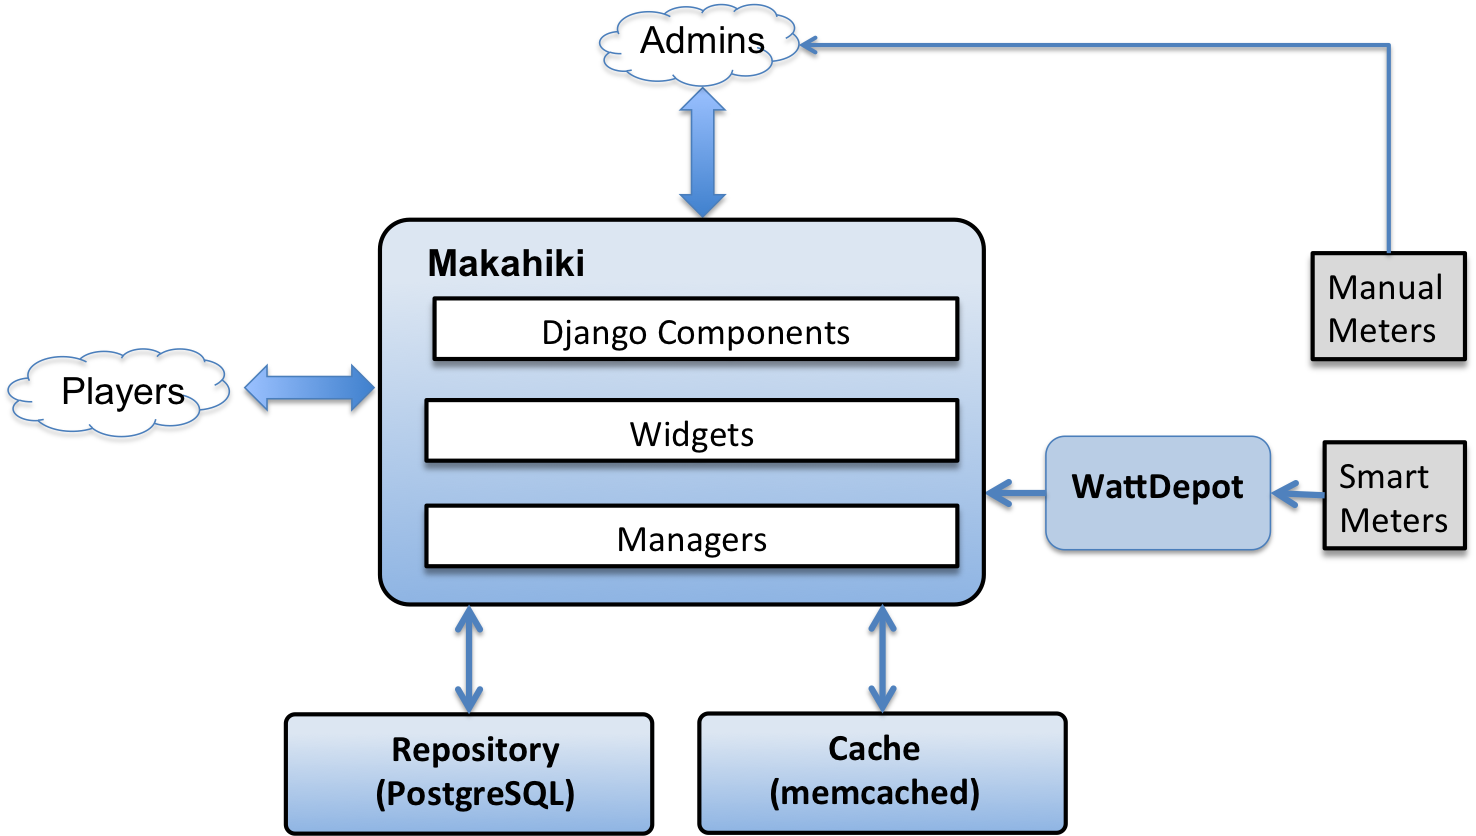
\includegraphics[scale=0.4]{system-architecture.png}
		\caption{Architecture of Makahiki}
	 	\label{fig:makahiki-architecture}
\end{figure}

\section{Experimental Design}

In order to evaluate how the Makahiki meets the research goals, we propose to investigate the following the research questions: \\

	(a) Can Makahiki be successfully deployed in multiple organizational scenarios to provide games for major sustainability issues (energy, water, waste, recycling, transportation, etc.)? \\

	(b) Can Makahiki provide an API and procedures to support enhancement with new features and capabilities with a minimum of impact on other aspects of the framework?\\
      
         (c) Can Makahiki provide an engaging and fun learning user interface to its end users?\\

	(d) Can Makahiki provide a mean to perform research on games for sustainability through A/B testing?\\

\subsection{Site Admin Evaluation}
To evaluate question (a), we plan to perform the case study research on multiple case studies. We call it ``Site Admin Evaluation''. It consists of surveys/interviews of administrators of all sites, asking for their assessment of the framework, whether it fulfilled their needs, and what they wish was different/better.

\subsection{Developer Evaluation Case Study}
To evaluate question (b), we plan to perform the case study research on at least one case. We call it ``Developer Evaluation". It consists of a ``case study'' of an external developer who is tasked with making an enhancement to the system.  Careful records of his interactions with developers, commits, and self-reported issues and problems along with interview data is used to determine how well the system achieved its goal as an extensible framework.

\subsubsection{Goal}
\begin{itemize}
  \item how easy it is to setup the development environments.
 \item how long did it take
 \item how easy it is to learn the system to understanding the architecture and existing functionalities.
 \item how easy it is to develop a new widget, testing, integration, documentation, packaging
\end{itemize}

\subsubsection{Data Collected}
\begin{itemize}
 \item time taken to setup the development env
 \item errors encountered
 \item helps from internal developers
 \item time spent in reading the doc initially
 \item time spent in reading the doc during the development
 \item time taken to create the initial revision
 \item time taken for unit testing, debugging
 \item time taken to integrate into the system
 \item number of makahiki APIs used
 \item commits, interactions in Github
\end{itemize}

\subsubsection{Data Collection Method and Protocol}
\begin{itemize}
\item interview log
\item meeting log
\item developer logbook
\end{itemize}

\subsection{End User Evaluation}
To evaluate question (c), we plan to perform end users data collection and analysis using the framework itself. We call it ``End User Evaluation". It consists of (1) in-game surveys of participants of all sites asking for their assessment of the game experience and its suitability to their situation;
(2) aggregated analytics data from log files of all sites, providing insight into what parts of site were used in what ways.

\subsection{A/B Testing Evaluation}
To evaluate question (d), we plan to perform the case study research on at least one case. We call it ``A/B Testing Evaluation". It consists of a ``case study" of one A/B test performed in Fall 2012 in order to answer the following research question: What level of energy data "latency" is required to provide useful feedback to participants in energy challenges like the Kukui Cup?  To assess this, we will implement three levels of energy latency in Fall 2012:  (1) Subminute-level latency through the Power Meter at HPU; (2) Hour-level latency through the Daily Energy Goal Game at UH (no Power Meter); and (3) Day-level latency through the manual Daily Energy Goal Game (at EWC).  In-game surveys can be used at each site to determine how much participants interacted with the given type of feedback, and whether they felt limited by the given level of latency.
  
%% Use this for an alphabetically organized bibliography
%%\bibliography{sustainability,csdl-trs,gamification}
%%\bibliographystyle{plain}

\end{document}
